\documentclass[12pt]{article}

\usepackage{ifxetex,ifluatex}

\ifnum 0\ifxetex 1\fi\ifluatex 1\fi=0 % if pdftex
  \usepackage[T1]{fontenc}
  \usepackage[utf8]{inputenc}
\else % if luatex or xelatex
  \ifxetex
    \usepackage{mathspec}
    \usepackage{xltxtra,xunicode}
  \else
    \usepackage{fontspec}
  \fi
  \defaultfontfeatures{Mapping=tex-text,Scale=MatchLowercase}
  \newcommand{\euro}{€}
\fi

\usepackage{amssymb,amsmath}
\usepackage{float}
\usepackage{fixltx2e} % provides \textsubscript
\usepackage{fancyhdr}
\usepackage[utf8]{inputenc}
\usepackage[T1]{fontenc}
\usepackage[portuguese]{babel}
\usepackage{graphicx}
\usepackage{indentfirst}
\usepackage{lipsum}
\usepackage{longtable}
\usepackage{pdfpages}
\usepackage[colorlinks=true,urlcolor=blue,citecolor=blue,linkcolor=blue]{hyperref}
\renewcommand{\familydefault}{\sfdefault}
\renewcommand{\baselinestretch}{1.4}

% Paper style
\usepackage[
  paperwidth=21cm,paperheight=29.7cm, % larger paper
  layoutwidth=21cm,layoutheight=27.82cm, % A4 landscape
  layouthoffset=0cm,layoutvoffset=1cm, % 1cm to crop on all sides
  left=2cm,right=2cm,top=2cm,bottom=2cm,
  headsep=\dimexpr3cm-72pt\relax,
  headheight=72pt]{geometry}

\pagestyle{fancy}
\lhead{}
\chead{}
\rhead{
\includegraphics[scale = 1]{logo-abj.png}}
\lfoot{}
\cfoot{Associação Brasileira de Jurimetria \\ Rua Gomes de Carvalho, 1356, 2º andar. CEP 04547-005 - São Paulo, SP,
Brasil \\ \url{http://abj.org.br}}
\rfoot{\text{} \\ \text{} \\ \thepage}
\renewcommand{\headrulewidth}{0.4pt}
\renewcommand{\footrulewidth}{0.4pt}


% Header information
\title{Análise TRF e TJ}
\author{}

\providecommand{\tightlist}{%
  \setlength{\itemsep}{0pt}\setlength{\parskip}{0pt}}

\begin{document}

\maketitle

\thispagestyle{fancy}

{
\hypersetup{linkcolor=black}
\setcounter{tocdepth}{2}
\tableofcontents
}
\pagebreak

\section{Levantamento das coletas sobre os
tribunais}\label{levantamento-das-coletas-sobre-os-tribunais}

Os tribunais requisitados para esta apresentação foram os TRFs e TJs,
entre eles,

\begin{enumerate}
\def\labelenumi{\arabic{enumi}.}
\item
  TRF

  \begin{enumerate}
  \def\labelenumii{\alph{enumii})}
  \item
    TRF-1
  \item
    TRF-2
  \item
    TRF-3
  \item
    TRF-5
  \end{enumerate}
\item
  TJ

  \begin{enumerate}
  \def\labelenumii{\alph{enumii})}
  \item
    TJSP
  \item
    TJAL
  \item
    TJDFT
  \item
    TJRJ
  \end{enumerate}
\end{enumerate}

Alguns deles não estão na análise, pois foram retirados para realizar
uma coleta mais consistente, como por exemplo, o TRF-2 ou tiveram
problemas na coleta como TJRJ. Além disso, cabe destacar que o caso do
TRF-5 precisa ser discutido, pois a maioria das decisões não são capazes
de informar o arquivamento ou não dos casos (irei explorar este caso ao
longo do relatório).

\section{TRF (Tribunal Regional
Federal)}\label{trf-tribunal-regional-federal}

\subsection{TRF-1}\label{trf-1}

\begin{verbatim}
1. Número de processos em segunda instância levantados.
\end{verbatim}

\textbf{315}

\begin{verbatim}
2. Taxa de arquivamento nos processos de segunda instância
\end{verbatim}

Para obter a taxa de arquivamento nos processos, basta procurar, por
meio de regex, palavras que podem estar relacionadas com tal ação. As
palavras escolhidas e suas variações foram, -\emph{rejeitar},
\emph{declarar extinta} e \emph{arquivou}.

Sendo assim a taxa de arquivamento no TRF-1 foi de \textbf{53,7\%}.

\subsection{TRF-2}\label{trf-2}

Nova coleta em andamento.

\subsection{TRF-3}\label{trf-3}

\begin{verbatim}
1. Número de processos em segunda instância levantados.
\end{verbatim}

\textbf{138}

\begin{verbatim}
2. Taxa de arquivamento nos processos de segunda instância
\end{verbatim}

Para obter a taxa de arquivamento nos processos, basta procurar, por
meio de regex, palavras que podem estar relacionadas com tal ação. As
palavras escolhidas e suas variações foram, -\emph{rejeitar},
\emph{declarar extinta} e \emph{arquivou}.

Sendo assim a taxa de arquivamento no TRF-3 foi de \textbf{52,9\%}.

\subsection{TRF-5}\label{trf-5}

\begin{verbatim}
1. Número de processos em segunda instância levantados.
\end{verbatim}

\textbf{857}

\begin{verbatim}
2. Taxa de arquivamento nos processos de segunda instância
\end{verbatim}

Para obter a taxa de arquivamento nos processos, basta procurar, por
meio de regex, palavras que podem estar relacionadas com tal ação. As
palavras escolhidas e suas variações foram, -\emph{rejeitar},
\emph{declarar extinta} e \emph{arquivou}.

Sendo assim a taxa de arquivamento no TRF-5 foi de \textbf{0,2\%}. O
resultado se dá devido a forma como o dado está disponível. A lista
abaixo mostra como e quantas decisões aparecem na base:

\begin{itemize}
\item
  À unanimidade, em preliminar, firmar a competência do TRF/5ª
  Reg\ldots{} - 1
\item
  DECIDE O PLENÁRIO DO TRF, POR UNANIMIDADE, REJEITAR A DENÚ\ldots{} - 1
\item
  MAIORIA, rejeitar a preliminar de incompetência da Justiça
  Feder\ldots{} - 1
\item
  POR MAIORIA - 135
\item
  POR MAIORIA, INDEFERIR A PRELIMINAR DE INCOMPETÊNCIA, E, À
  UNANI\ldots{} -1
\item
  POR UNANIMIDADE, ACOLHER A PRELIMINAR DE INCOMPETÊNCIA
  ABSOLUTA\ldots{} -1
\item
  POR UNANIMIDADE, DECLINAR DA COMPETÊNCIA EM FAVOR DA JUSTIÇA
  FED\ldots{} -1
\item
  POR UNANIMIDADE, DECLINAR DA COMPETÊNCIA, E POR MAIORIA,
  DETERMI\ldots{} -1
\item
  Por unanimidade, receber a denúncia, e, por maioria,
  determinar\ldots{} -1
\item
  POR UNANIMIDADE, RECEBER A DENÚNCIA, POR MAIORIA, DETERMINOU O
  E\ldots{} -1
\item
  UNÂNIME - 713
\end{itemize}

\subsection{Visualização gráfica}\label{visualizacao-grafica}

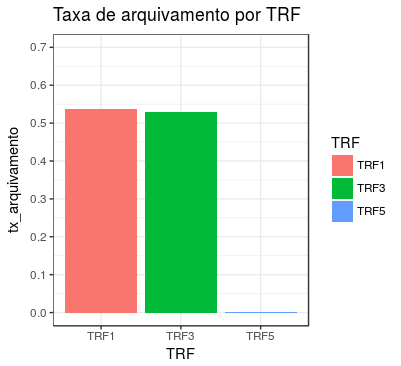
\includegraphics[width=5.57in]{plot_trf}

\section{TJ (Tribunal de Justiça)}\label{tj-tribunal-de-justica}

\subsection{TJSP}\label{tjsp}

\begin{verbatim}
1. Número de processos em segunda instância levantados.
\end{verbatim}

\textbf{1001}

\begin{verbatim}
2. Taxa de arquivamento nos processos de segunda instância
\end{verbatim}

Para obter a taxa de arquivamento nos processos, basta procurar, por
meio de regex, palavras que podem estar relacionadas com tal ação. As
palavras escolhidas e suas variações foram, -\emph{rejeitar},
\emph{declarar extinta} e \emph{arquivou}.

Sendo assim a taxa de arquivamento no TJSP foi de \textbf{76,2\%}.

\subsection{TJAL}\label{tjal}

\begin{verbatim}
1. Número de processos em segunda instância levantados.
\end{verbatim}

\textbf{8}

\begin{verbatim}
2. Taxa de arquivamento nos processos de segunda instância
\end{verbatim}

Para obter a taxa de arquivamento nos processos, basta procurar, por
meio de regex, palavras que podem estar relacionadas com tal ação. As
palavras escolhidas e suas variações foram, -\emph{rejeitar},
\emph{declarar extinta} e \emph{arquivou}.

Sendo assim a taxa de arquivamento no TJAL foi de \textbf{37,5\%}.

\subsection{TJDFT}\label{tjdft}

\begin{verbatim}
1. Número de processos em segunda instância levantados.
\end{verbatim}

\textbf{80}

\begin{verbatim}
2. Taxa de arquivamento nos processos de segunda instância
\end{verbatim}

Para obter a taxa de arquivamento nos processos, basta procurar, por
meio de regex, palavras que podem estar relacionadas com tal ação. As
palavras escolhidas e suas variações foram, -\emph{rejeitar},
\emph{declarar extinta} e \emph{arquivou}.

Sendo assim a taxa de arquivamento no TJDFT foi de \textbf{45\%}.

\subsection{Visualização gráfica}\label{visualizacao-grafica-1}

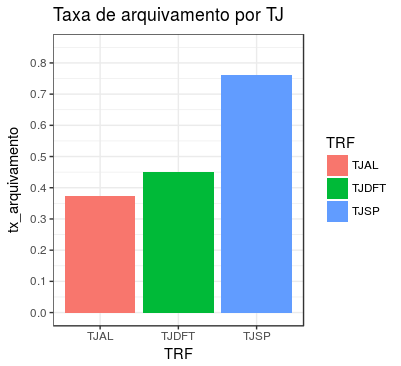
\includegraphics[width=5.57in]{plot_tj}

\end{document}
